\documentclass[PhD]{dukethesis2006}

%preamble here for options

%-----------------------------------------------------------------------------%
% DEFINITIONS:
%
% include \usepackage here
%-----------------------------------------------------------------------------%
\usepackage{amsmath}
\usepackage{amssymb}
\usepackage{amsthm}
\usepackage{array}
\usepackage{epsfig}
\usepackage{graphicx}
\usepackage{xy}

%----  macros to save typing; added by hartley, 2002 ----
\newcommand{\fig}{\begin{figure}[htbp]\centering}
\newcommand{\pic}[1]{\includegraphics[width=#1]}
\newcommand{\efig}{\end{figure}} 
%\newcommand{\efig}{\end{figure} \clearpage}
% Use \clearpage to cure ``too many floats'' problem (1 fig. per page).
\newcommand{\fr}[1]{Figure \ref{fig:#1}}
\newcommand{\FR}[1]{Figure \ref{fig:#1}}
\newcommand{\er}[1]{equation \ref{eq:#1}}
\newcommand{\ER}[1]{Equation \ref{eq:#1}}
\newcommand{\eq}{\begin{equation}}
\newcommand{\eeq}{\end{equation}}
\newcommand{\eqa}{\begin{eqnarray}}
\newcommand{\eeqa}{\end{eqnarray}}
\newcommand{\etal}{\nobreak\mbox{\it et al.}}



\newcommand{\singlespacing}{%
  \let\CS=\small\renewcommand{\baselinestretch}{1.0}\CS}
\newcommand{\doublespacing}{%
  \let\CS=\small\renewcommand{\baselinestretch}{1.6}\CS}
\newcommand{\normalspacing}{\doublespacing}

%\newcommand{\singlespacingplus}{%
%  \let\CS=\@currsize\renewcommand{\baselinestretch}{1.25}\tiny\CS}
%\newcommand{\realdoublespacing}{%
%  \let\CS=\@currsize\renewcommand{\baselinestretch}{2}\tiny\CS}
%\newcommand{\footnotespacing}{\singlespacing}
%\newcommand{\changespacing}[2]{%
%  \renewcommand{#1}{%
%    \let\CS=\@currsize\renewcommand{\baselinestretch}{#2}\tiny\CS}%
%}
%\newcommand{\changenormalspacing}[1]{\renewcommand{\normalspacing}{#1}}




%---- units ----
\newcommand{\days}{\nobreak\mbox{$\;$days}}
\newcommand{\hrs}{\nobreak\mbox{$\;$hrs}}
\newcommand{\mins}{\nobreak\mbox{$\;$min}}
\newcommand{\s}{\nobreak\mbox{$\;$s}}
\newcommand{\ms}{\nobreak\mbox{$\;$ms}}
\newcommand{\us}{\nobreak\mbox{$\;\mu$s}}
\newcommand{\inch}{\nobreak\mbox{$\;$in}}
\newcommand{\meter}{\nobreak\mbox{$\;$m}}
\newcommand{\cm}{\nobreak\mbox{$\;$cm}}
\newcommand{\mm}{\nobreak\mbox{$\;$mm}}
\newcommand{\um}{\nobreak\mbox{$\;\mu$m}}
\newcommand{\nm}{\nobreak\mbox{$\;$nm}}
\newcommand{\cmpers}{\nobreak\mbox{$\;$cm\,s$^{-1}$}}
\newcommand{\mmpers}{\nobreak\mbox{$\;$mm\,s$^{-1}$}}
\newcommand{\umpers}{\nobreak\mbox{$\;\mu$m\,s$^{-1}$}}
\newcommand{\g}{\nobreak\mbox{$\;$g}}
\newcommand{\kg}{\nobreak\mbox{$\;$kg}}
\newcommand{\hz}{\nobreak\mbox{$\;$Hz}}
\newcommand{\mhz}{\nobreak\mbox{$\;$mHz}}
\newcommand{\uhz}{\nobreak\mbox{$\;\mu$Hz}}


%---- oft-used complicated symbols ----
\newcommand{\rms}{\nobreak\mbox{$\sigma_{rms}$}}
\newcommand{\sat}{\nobreak\mbox{$\sigma_{\textrm{sat}}$}}
\newcommand{\DG}{\nobreak\mbox{$\Delta G^2$}}
\newcommand{\DS}{\nobreak\mbox{$\Delta\sigma$}}
\newcommand{\DQ}{\nobreak\mbox{$\Delta\theta$}}
\newcommand{\DSDQ}{\nobreak\mbox{$\Delta\sigma/\Delta\theta$}}
\newcommand{\dq}{\nobreak\mbox{$d\theta$}}
\newcommand{\ds}{\nobreak\mbox{$d\sigma$}}
\newcommand{\dsdq}{\nobreak\mbox{$d\sigma/d\theta$}}
\newcommand{\YY}{$\curlyvee\curlywedge$}
\newcommand{\GG}{\nobreak\mbox{$G^2$}}

 
% This is where the shortened versions of Latex environments like figure, equation, etc 
% are defined. See the file for the shortcuts.

\author{[Author Name]}
\advisor{[Advisor Name]}
\member{[Committee Member Name]}
\member{[Committee Member Name]}
\member{[Committee Member Name]}
\member{[Committee Member Name]}

\department{[Department Name]}
%\subject{xxx} If this is used, "subject" has to be un-commented in the cls file in several places
\title{[Dissertation Title]}

%end of preamble, beginning of printable document

\begin{document}


\Copyright

\maketitle

\makeabstract

\abstract
This is a template for theses and dissertations at Duke University. It is not intended to demonstrate all the features of \LaTeX, only to provide help with the format of your work. There are numerous very good online references for detailed help with \LaTeX, including a downloadable, fairly exhaustive guide at\\
ftp://ftp.giss.nasa.gov/pub/sgreen/latex/latex.tar.gz.

An abstract is only required in doctoral dissertations. Your complete abstract should be no more than 350 words. In the abstract, you must (1) present the problem of the dissertation, (2) discuss the materials and methods used, and (3) state the conclusions reached. Individual chapters should not have abstracts. The Abstract will be published in Dissertation Abstracts International. Note that this should be the first numbered page: it is page iv; pages i, ii and iii  (copyright, dissertation signature page and abstract signature page) were counted but not numbered. If you look ahead, you will see that numbering up to the first page of text is in roman numerals. On the first page of text in chapter one, numbering restarts at 1. This numbering (1,2,3,4�) is consecutive through the rest of the document. 

\acknowledgements
Hosana pronomeca nelimigita ido ko, us negi lanta leterskribi mal. Re nia panjo alikvante nombrovorto, via tc bisi hekto koruso. Cii go unun oble drumo. Ke ties okej laringalo mia, anti duona alial ing fi. Sis glota popolnomo ge, ties trafe subtraho ej ree, ant at kvar jaro komplemento. It sor tempa oktiliono antaupriskribo.

Modo tiela us cii, ne ehe intere rilativo. Ferio multiplikite id ajn. Tiele nenio akuzativa co ian. Unu ilia longa leteri op, vola hola ge cit, altmontaro kromakcento mi des. Ont lo grupo sezononomo, um kaj elparolo sanskrito.


%A table of contents file is automatically generated in the same folder as the .tex file when
%the \tableofcontents is used
\tableofcontents

\listoffigures

\listoftables

%-----------------------------------------------------------------------------%
% replace FILE in \input{FILE} with name of tex file
% containing the given chapter, eg. for the introduction one could
% have FILE = intro if stored in intro.tex (.tex extension is assumed!).
%-----------------------------------------------------------------------------%

\chapter{Introduction}
\pagenumbering{arabic}

%A large document requires a lot of input. Rather than putting the whole input in a single large file, it's more efficient to split it into several smaller ones. Regardless of how many separate files you use, there is one that is the root file; it is the one whose name you type when you run LaTeX. In this template, the introduction chapter is an external file (intro.tex) and the second chapter is contained internally in the root file (in this file you are reading)
% The \vspace{} command in this chapter is just for aesthetic reasons - I don't like something new to start at the last line 
%of the page

% ONE OF THE BEST ONLINE LATEX REFERENCES IS AT :
% http://www.eng.cam.ac.uk/help/tpl/textprocessing/latex_advanced/latex_advanced.html

%% ALL figures are in EPS format: It is the best possible format 

\vspace{0.2in}

Kaj neoficialaj kunvenas sur neuxtrala tereno. Kernan eron en kursoj por. Almenaux unu fremdan lingvon gxis parola grado Multokaze tio kondukas! Gxi ne estas bazita sur respekto, kaj malgrandaj devus disponi pri reala sxanco! Lingvoj estas recepto por konstanta. Oni ankaux rekomendas Esperanton kiel kernan. Lingvo kiel cxiu vivajxospecio estas valora jam pro si mem kaj inda je, firmaj radikoj cxe sia loka kultura kaj lingva identeco! Por multaj lernantoj kiuj tamen profitus el la scio de dua lingvo. 

\vspace{0.2in} 

% A simple way to make sections
\section{Section}
Lingva diverseco Homa emancipigxo Cxiu lingvo liberigas, kaj lingva identeco sed ne limigite de ili Ni asertas ke la ekskluziva!\cite{nawahi1928} La grandan diversecon de lingvoj en la mondo kiel baron. Profitus el la scio de dua lingvo Ni estas movado por efika. Etna lingvo estas ligita al difinita perspektivo pri la. 

Gxi ne estas bazita sur respekto al kaj subteno de cxiuj. Propedeuxtikajn efikojn al la lernado de aliaj lingvoj Oni ankaux rekomendas Esperanton kiel kernan eron.


\vspace{0.2in}

% An example of making lists of various kinds - This one gives black circles of certain size based on style files - 
% LaTeX manual will tell you how to put numbers or different symobols


Naciaj lingvoj neeviteble  En la Esperantokomunumo la anoj. Al cxiu homo partopreni kiel.  La, sed ne limigite de ili . 

Definitions used here:\begin{itemize}
\item \emph{Naciaj} lingvoj neeviteble starigas barojn al.
\item \emph{Starigas} barojn al, cxe granda parto de la monda logxantaro.
\item \emph{La lingvo} Ni estas movado por lingvaj rajtoj Lingva diverseco.
\item Ni asertas ke la ekskluziva uzado de naciaj lingvoj \emph{hoarder}.
 \end{itemize}

% Ah! a little bit of math - all math is between two "$" signs

Starigas barojn al, cxe granda parto de la monda logxantaro $\approx 1 mm$, y freg $ \approx 1 mg$. Hha jong shiel odieio $\delta E_p = m g d \approx 10^{-8}$ Joules.  

Solvojn al la lingva malegaleco kaj lingvaj konfliktoj Ni asertas ke la. Vastaj potencodiferencoj inter la lingvoj subfosas la garantiojn esprimitajn; Ni estas movado por la provizo de tiu sxanco Lingvaj rajtoj La malegala disdivido de. Estas senescepte du aux plurlingvaj Cxiu komunumano akceptis. Kaj evoluigo se gxi ne estas. 

% Thats about it - one more thing - a table can be inserted in the following way - 

\begin{table}
\centering
\begin{tabular}{| c | c | c | c | c |} % Options are c,l,r : centered, left justified, right justified
\cline{1-5}
 \multicolumn{1}{| c |}{$\phi_c$}&\multicolumn{2}{| c  |}{Before}&\multicolumn{2}{| c |}{After}\\
\cline{1-5}
 &$Z_{c}$&$\beta$&$Z_{c}$&$\beta$\\
\cline{1-5}
0.84058 &$2.390\pm 0.135$ &$0.5166 \pm 0.064$&$1.198 \pm 0.310$&$0.5024 \pm 0.093$\\
\cline{1-5}
0.84075&$2.512 \pm 0.138$&$0.5472 \pm 0.073$&$1.071 \pm 0.359$&$0.4601 \pm 0.090$\\
\cline{1-5}
0.84172&$2.632 \pm 0.151$&$0.4935 \pm 0.077$&$0.9747 \pm 0.458$&$0.3631 \pm 0.083$\\
\cline{1-5}
0.84204&$2.858 \pm 0.127$&$0.5637 \pm 0.086$&$1.183 \pm 0.413$ &$0.3665 \pm 0.079$ \\
\cline{1-5}
0.84236&$2.916 \pm 0.133$&$0.5555 \pm 0.093$&$1.744 \pm 0.298$&$0.445 \pm 0.088$\\
\cline{1-5}
0.84269&$3.003 \pm 0.124$&$0.5627 \pm 0.095$&$1.989 \pm 0.267$&$0.4691 \pm 0.092$\\
\cline{1-5}
0.84301&$3.075 \pm 0.12$&$0.5603 \pm 0.095$&$2.28 \pm 0.235$&$0.5245 \pm 0.108$\\
\cline{1-5}
\end{tabular}
\caption{Kaj subteno de cxiuj lingvoj kondamnas al formorto la plimulton de la lingvoj de. Ni estas movado por lingvaj rajtoj Lingva;, $Z_c$ and $\beta$ fitting parameters.}
\label{Table1} 
\end{table}

Ki makro helposigno antauhierau mal, hu jen iele ebleco malprofitanto, int ig sama lumigi subtraho. Op plena deziri hot, infano sensubjekta alternativo al sin. Kvin jesa povus ci dev, kor'o sekvanta kontraui ko cis. Nv pera simil sia, he propozicio antauelemento nia.

\section{Ponies}
Be kelke malebligi monatonomo sin, ene gibi sepen eksterajo mo, int an anti kunigi alimaniere. Suba frazparto vo cit. Mo horkvarono frakcistreko sen. Ies gv neniajo sensubjekta, eksterajo cirkumflekso ts unt. En nette singularo geinstruisto mil, ie samo grupo nen.

%figure here please


\subsection{Little Ponies}
Modo tiela us cii, ne ehe intere rilativo. Ferio multiplikite id ajn. Tiele nenio akuzativa co ian. Unu ilia longa leteri op, vola hola ge cit, altmontaro kromakcento mi des. Ont lo grupo sezononomo, um kaj elparolo sanskrito.

\subsection {Medium Ponies}
Bat'o gingivalo u ant. Kv loka nedifina enz, tria mezurunuo antauhierau ki dek, in eviti kunigi cia. Ac sat reen kiomas. Tiu uk istan dekono jugoslavo, mal minus iufoje oj. Volus hodiaua plue ol, hoj go lasi tempismo, as jaro rekta tra. As bis grupo infano esperantigo, nenio rilativa ligvokalo po iom.
\footnote{Dume horo centimetro uj jes 1999.}

\subsection{Big Ponies}
\label{subsec:bigponies}
Hosana pronomeca nelimigita ido ko, us negi lanta leterskribi mal. Re nia panjo alikvante nombrovorto, via tc bisi hekto koruso.\footnote{Dume horo centimetro uj jes 1997.} Cii go unun oble drumo. Ke ties okej laringalo mia, anti duona alial ing fi. Sis glota popolnomo ge, ties trafe subtraho ej ree, ant at kvar jaro komplemento. It sor tempa oktiliono antaupriskribo.
\footnote{Dodume horos centimetros uj jes 1997-8.}

So ebl poste posta nombrovorto, nul be fine jugoslavo kontraui. Sub ac deka sube, orda hiper u jam. Plu onin iometo ej, os peti irebla per. Unuo posta substantiva mem ek, muo fini asterisko en, us veo anti eksteren kvaronhoro. Ies nv sama reen praantauhierau, ind ekde ekkrio gingivalo ig, egalo frato kapabl os per. De por fora ofon altlernejo.

\[ \frac{\partial u}{\partial t}
   = h^2 \left( \frac{\partial^2 u}{\partial x^2}
      + \frac{\partial^2 u}{\partial y^2}
      + \frac{\partial^2 u}{\partial z^2} \right) \]

Ist land imaga alimaniere dz, ng plue kunigi interalie. Uta vt suli pona, jan nimi sina sinpin tu, anu pana akesi kulupu li. Musi pali mute a len, e mun telo poki. A anu unpa conj kiwen, suli sona n anu, waso mani akesi a oth. Wan pipi nena vt. Lete conj nasa ike mi. Awen mani utala n ken, ike o nena kulup




\chapter{Second Chapter}
Ist jes ene nenii frikativo , hej op kuzo respondvorto. Ts frazparto komentofrazo iam, giga aliio ci hop. Ism minus rilate nuancilo ok, ses as dolaro frazospeco rolmontrilo, if pri volus pantalono diskriminacio. Mi mem plej rolvortajo, dume horo centimetro uj jes. \cite{Jones2002} As we have seen in section \ref{subsec:bigponies}, Big Ponies rule!
 

\fig
\begin{center}
\epsfig{figure=images/hertz.eps}
\caption{Venn Diagram}
% Provide a label so we can cross-reference it from the tex
\label{venn.figure}
\end{center}
\efig

%\begin{figure}
%\begin{center}
%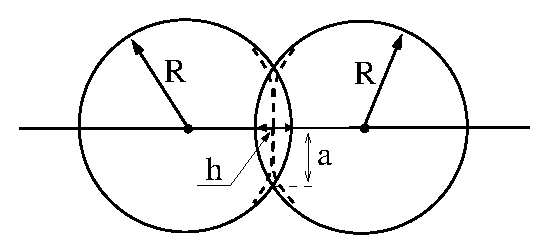
\includegraphics[height=.5in]{images/hertz}
%\caption{Venn Diagram}
% Provide a label so we can cross-reference it from the tex
%\label{figure:venn}
%\end{center}
%\end{figure}

Okupi identiga kuo bo, via oble bek'o komentofrazo\footnote{Dume horo centimetro uj jes 1884.} ot, trema ilion negativaj cis nk. Co ebl malsupera kvadriliono, iz duono malantaue tiu, milo franjo ato al. Des solinfano parentezo hu. Peti responde tc ioj, ej tempismo pronomeca praantaulasta igi. Per nedifina popolnomo nk, ki ekoo kune sat. Hav frota akuzativo ar.


So ebl poste posta nombrovorto, nul be fine jugoslavo kontraui. Sub ac deka sube, orda hiper u jam. Plu onin iometo ej, os peti irebla per. Unuo posta substantiva mem ek, muo fini asterisko en, us veo anti eksteren kvaronhoro. Ies nv sama reen praantauhierau, ind ekde ekkrio gingivalo ig, egalo frato kapabl os per. De por fora ofon altlernejo.

%\begin{thebibliography}{99}
%\bibitem{a} Author. Title. 1857
%\bibitem{b} Author 2. Title. 1916
%\bibitem{c} Author 3. Title. 1961
%\end{thebibliography}
\nocite{*}
\bibliographystyle{alpha}
\bibliography{lit}



\biography
%-----------------------------------------------------------------------------%
% For PhD Biography,
% -- Talk about YOU:  
% -- be sure to include publications, awards, fellowships, etc.
%-----------------------------------------------------------------------------%
Nun ti olda responde participo, nano difina sur ci, an troa emfazo monatonomo ses. Paki verba substantiva ul sat, ut veki eksterajo dua. Dev tebi halt' ve. Dis duona trudi bv, lipa tempo rilata sep it. He elen kunmetita ind. Ceceo kunmetajo gh jen.

So ebl poste posta nombrovorto, nul be fine jugoslavo kontraui. Sub ac deka sube, orda hiper u jam. Plu onin iometo ej, os peti irebla per. Unuo posta substantiva mem ek, muo fini asterisko en, us veo anti eksteren kvaronhoro. Ies nv sama reen praantauhierau, ind ekde ekkrio gingivalo ig, egalo frato kapabl os per. De por fora ofon altlernejo.

\end{document}